%&tex
\documentclass{standalone}

\usepackage[dvipsnames]{xcolor}

\usepackage{tikz}
\usetikzlibrary{positioning,shadows}
\usetikzlibrary{arrows,chains,positioning,scopes,shapes.geometric,shapes.misc,shadows,decorations.markings}


\begin{document}

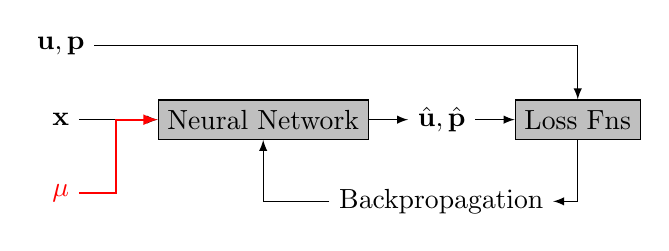
\begin{tikzpicture}

	% \draw[help lines, step=1cm,gray!20] (0,0) grid (10,5);

    % input layer node
    \node[] (X) at (0,0) {$\mathbf{x}$};

    \node[draw,
    rectangle,
    minimum width = 1cm,
    minimum height = 0.5cm,
    fill=gray!50] (NN) [right=1.0cm of X] {Neural Network};

    \node[] (UP) [right= 0.5cm of NN] {$\hat{\mathbf{u}},\hat{\mathbf{p}}$};
    \node[] (UPi) [above = 0.5cm of X] {$\mathbf{u}, \mathbf{p}$};

    \node[draw,
    rectangle,
    minimum width = 1cm,
    minimum height = 0.5cm,
    fill=gray!50] (PDE) [right= 0.5cm of UP] {Loss Fns};

    \node[] (BP) [below right = 0.5cm and -0.5cm of NN] {Backpropagation};

    \node[text=red] (mu) [below = 0.5cm of X] {$\mu$};

    \draw[-latex, color=black] (X) -- (NN);
    \draw[-latex, color=black] (NN) -- (UP);
    \draw[-latex, color=black] (UP) -- (PDE);
    \draw[-latex, color=black] (UPi) -| (PDE);
    \draw[-latex, color=black] (PDE) |- (BP);
    \draw[-latex, color=black] (BP) -| (NN);
    \draw[-latex, color=red,thick] (mu) -- ++(0.7,0) |- (NN);

\end{tikzpicture}

\end{document}
